\subsection{SmARt World}
\label{sec:smart}

	\textit{SmARt World} é um \textit{framework} voltado para a computação ubíqua, ao qual utiliza a 
	Realidade Aumentada com o objetivo de criar novos conteúdos virtual e interação com o ambiente
	inteligente~\cite{yew}. Outro objetivo desse \textit{framework} está no auxílio da construção de
	aplicações voltada para a Realidade Aumentada baseada em dispositivos móveis, tornando esse
	desenvolvimento simplificado. O \textit{framework} é capaz de criar e apresentar objetos virtuais
	ao usuário, provendo uma interação por meio destes. Sua arquitetura é dividida em: 
	
	%Sua arquitetura é ilustrada conforme a
	%figura~\ref{fig:arquitetura_smart}.
	
	%\begin{figure}[htb]
	%	\centering 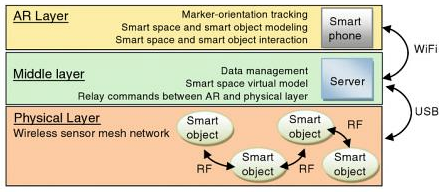
\includegraphics[scale=0.8]{figuras/cap2/arquitetura_smart.png}
	%	\caption{\textit{Arquitetura do framework SmARt World \cite{yew}.}}
	%	\label{fig:arquitetura_smart}
	%\end{figure}
	
	\begin{enumerate}
	  \item \textbf{Camada Física}
	  	
	  	Nessa camada os objetos inteligentes são interligados através de transmissores de rádio
	  	frequência, onde estes são ligados um nó central que faz acesso a Camada Intermediária. Esse nó
	  	central também fica responsável por reconhecer os demais nós ativos na rede, controlar as
	  	informações que são repassadas pelos nós e posteriormente enviar os dados a Camada Intermediária
	  	para que as informações correspondentes aos nós sejam atualizadas.
	  	
	  	Cada transmissor possui seu código identificador para se comunicar com a rede, essa comunicação
	  	é feita através de sensores ou por comunicações interligadas fisicamente. O objetivo da
	  	utilização desses transmissores acoplados aos dispositivos possibilita o controle dos
	  	mesmos, acrescentando uma inteligência a rede. Desta forma, de acordo com a informação captada
	  	pelos transmissores, é possível enviar sinais específicos para os dispositivos. Esse controle
	  	será feito através da interface provida pelo~\textit{smartphone}, na Camada AR.
	  
	  \item \textbf{Camada Intermediária}
	  
	  	Essa camada possui a responsabilidade de armazenar e gerenciar todas as informações a respeito
	  	do ambiente inteligente e dos usuários e objetos pertencentes a ele. A comunicação entre a
	  	aplicação e os demais componentes da rede é feita através de uma interface web que
	  	disponibiliza acesso a aplicação e ao banco de dados contido em servidor. O banco de dados
	  	armazena informação a respeito do objeto, tais como: posicionamento, modelagem 3D, textos
	  	apresentados ao usuário, formato e contexto. 
	  
	  \item \textbf{Camada AR}
	
		Essa camada utiliza uma aplicação voltada para a Realidade Aumentada que é capaz de
		rastrear e reconhecer os marcadores. Através disso possibilita uma interação entre os
		objetos virtuais e reais. Essa camada foi projetada para ser utilizada em dispositivos móveis.
		Por essa razão, o protótipo para essa camada foi desenvolvido para a plataforma Android.
		
	\end{enumerate}
	
	\subsubsection{Marcadores e a Realidade Aumentada}
	
	O rastreamento e reconhecimento dos marcadores é feito a partir de dois métodos combinados. O
	primeiro é o reconhecimento dos objetos através do uso de marcadores. Após o reconhecimento, o
	segundo método é iniciado. Neste, sensores são utilizados para obter a orientação e posicionamento
	do objeto. Esse posicionamento é gravado na Camada Intermediária através das coordenadas \{x,y,z\}. O
	\textit{framework} possui a funcionalidade de seleção de objetos virtuais através da tela do
	\textit{smartphone}, possibilitando redefinir o novo posicionamento do objeto virtual selecionado
	no ambiente inteligente.
	
	
	